\documentclass[10pt,twocolumn]{article}
\usepackage[margin=0.9in]{geometry}
\usepackage{graphicx}
\usepackage{hyperref}
\usepackage{cite}


\title{\large{Spectral Clustring Based on Local PCA with Application to Hand-written Digit Separation}}
\author{
    Yu, Guangting\thanks{Quantitative Finance \& Risk Management, Department of Mathematics} \\
    \small{\texttt{yugtmath@umich.edu}}
    \and
    Jia, Guo\thanks{Applied \& Interdisciplinary Math Ph.D., Department of Mathematics} \\
    \texttt{guojia@umich.edu}
    \and
    Tsukamoto, Masaya\thanks{Quantitative Finance \& Risk Management, Department of Mathematics} \\
    \texttt{masayats@umich.edu}
    \and
    Wang, Zihan\thanks{Space Science Ph.D., Department of Climate and Space Sciences and Engineering} \\
    \texttt{wzihan@umich.edu}
}


\begin{document}
\maketitle

\subsection*{Problem statement}
\begin{figure}[htbp]
\centering
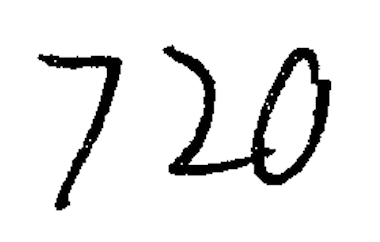
\includegraphics[width=0.1\textwidth]{connected-digits.png}
\hspace{1em}
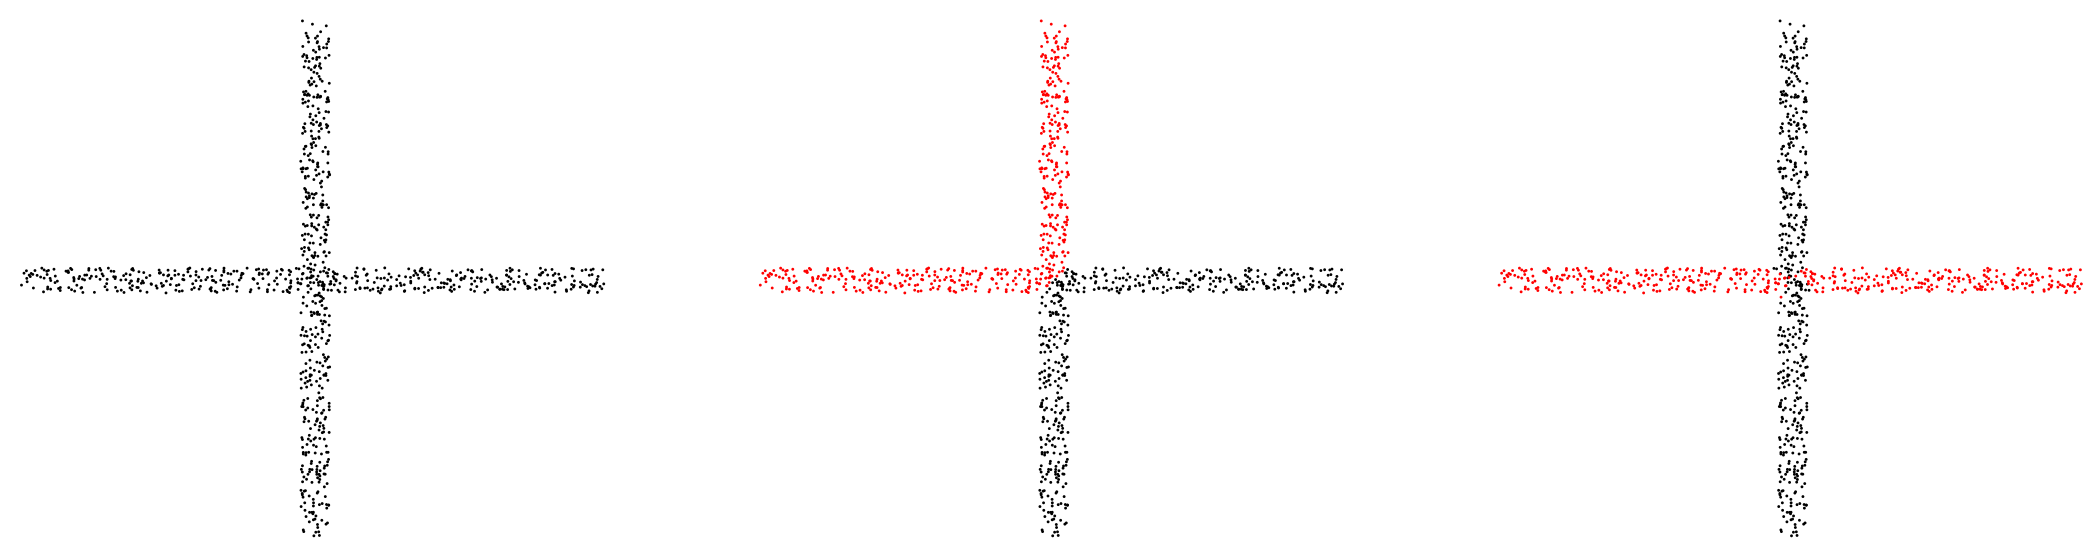
\includegraphics[width=0.3\textwidth]{effect.png}
\caption{(1) Connected digits, (2) sample pixels (3) spectral clustering by Ng. et al (2002), (4) spectral clustering by local PCA}
\label{fig1}
\end{figure}
In hand-written digit recognition, if the digits are connected, (like `2' and `0' in Figure \ref{fig1}), there is no chance for the classifier to output the correct result.
So we want to separate the connected digits apart.
\subsection*{Motivation}
This problem is motivated from one of the computer vision problem to recognize hand-written digits.
Many good algorithms have been developed to classify a single digit with very high accuracy.
However, when we switch to multiple digits, one of the difficulties is that if the digit accidentally intersect with each other
\subsection*{Papers to focus on}
We will focus on two papers, since one of the paper is published with the code.
The paper with \href{http://sciences.ucf.edu/math/tengz/wp-content/uploads/sites/45/2016/07/code.zip}{code} is
\href{http://www.jmlr.org/papers/volume18/14-318/14-318.pdf}{(Arias-Castro and Lerman, Zhang,2017)}
\cite{Arias-Castro:2017:SCB:3122009.3122018}
The other paper is \href{https://papers.nips.cc/paper/4246-sparse-manifold-clustering-and-embedding.pdf}{(Elhamifar and Vidal, 2011)}
\cite{NIPS2011_4246}, which is cited by \cite{Arias-Castro:2017:SCB:3122009.3122018} for comparison.
These authors also write some other papers related to spectral clustering, so they also be helpful in understanding the possible variations and extensions of the algorithm.


\subsection*{Methods to be compared}
We will compare the spectral clustering algorithms mentioned in these two papers with \href{https://papers.nips.cc/paper/2092-on-spectral-clustering-analysis-and-an-algorithm.pdf}{(Ng and Jordan, Weiss, 2001)}\cite{Ng:2001:SCA:2980539.2980649} which will be introduced in class.
One of the effect, as Arisa-Castro indicated, is that Ng's algorithm may detect non-smooth manifold, while the spectral clustering bases on local PCA can typically detect smooth manifolds as Figure \ref{fig1} shows.\cite{Arias-Castro:2017:SCB:3122009.3122018}


\subsection*{Data sets}
For hand-written digit separation, we will use self-generated test-cases (e.g., Figure \ref{fig1}).
The advantage of self-generated data set is that we can test specifically on the intersection and see if the spectral clustering gives the correct separation, and it is very convenient for small number of test-cases.
Another public library, MNIST, may be an option for stress testing, but we still need to pairwisely intersect them to produce the desired input.

Also, the spectral clustering algorithm is not restricted to hand-written digit recognition.
We can design other manifolds for the algorithm to detect.
Arias-Castro did the M\"{o}bius strips and paraboloids intersection separation \cite{Arias-Castro:2017:SCB:3122009.3122018}, and we can try Klein bottle or torus.

\subsection*{Group member roles}
\paragraph{Guangting Yu} will be responsible for algorithm implementation, code management, testing and comparing with similar algorithms.
\paragraph{Jia Guo} will be responsible for reading the proofs of theorems in the paper and conduct mathematical analysis on our implementation.
\paragraph{Masaya Tsukamoto} will be responsible for test-case designing, including hand-written digit generation and smooth intersecting manifolds for separation.
\paragraph{Zihan Wang} will be responsible for writing reports by joining all the work from teammates.

\newpage
\bibliography{reference}{}
\bibliographystyle{plain}
\end{document}